\documentclass[journal=jacsat,manuscript=article]{achemso}
\usepackage[version=3]{mhchem} 
\usepackage{gensymb}
\newcommand*\mycommand[1]{\texttt{\emph{#1}}}

\author{Harsh Agrawal}
\email{ha1822@ic.ac.uk}
\affiliation[Imperial College London]
{Department of Bioengineering, Imperial College London}

\title[Preparation and Study of Gold Nanorods and Quantum Dots]
  {Synthesis of Gold Nanorods via Seed Mediated Growth and Quantum Dots via Hot Injection Method}


\begin{document}

\begin{abstract}
  Quantum Mechanics is the primary governing principle at small length scales. The phenomena observed at these scales are different than that of the bulk material. Gold Nanorods and Quantum Dots are two such examples that demonstrate this behavior. Both Quantum Dots and Gold Nanoparticles are desired for their unique optoelectronic properties and are used widely in the domains of diagnostics, imaging, displays, etc. We conduct two experiments: one to study the effect of different seed concentrations on the formation of gold nanorods and the other on the effect of capping agents such as Oleyamine on forming quantum dots. We find that a higher concentration of seed solution leads to a higher yield of gold nanorods with similar size and aspect ratios. We also find that adding capping agents leads to a more uniform and monodisperse yield of quantum dots with lower UV luminescence properties.
\end{abstract}

%%%%%%%%%%%%%%%%%%%%%%%%%%%%%%%%%%%%%%%%%%%%%%%%%%%%%%%%%%%%%%%%%%%%%
%% Start the main part of the manuscript here.
%%%%%%%%%%%%%%%%%%%%%%%%%%%%%%%%%%%%%%%%%%%%%%%%%%%%%%%%%%%%%%%%%%%%%
\section{Seed Mediated Growth of Gold Nanorods}
Gold Nanorods work on the simple principle of Surface Plasmon Resonance\cite{huang2010gold}. When light is radiated onto gold nanorods, it excites the electrons to oscillate together at the same frequency as the incident light. This effect is greatest at the resonance frequency and these oscillations are known as surface plasmons. These plasmons, proportional to their excitation, transfer their energy to free electrons via photons thus causing absorption of light. Larger nanorods have higher wavelength plasmons and thus absorb light of lower energy and vice versa.

Gold nanorods can thus be prepared, and tuned for a proper size, to absorb light of a particular wavelength. The protocol for the production of seed-mediated growth of gold nanorods (of length 20 to 100nm) was first developed by Jana et.\ al.\cite{jana_et_al} The yield they obtained, however, was quite low as their protocol led to the collective synthesis of spherical gold nanoparticles along with nanorods. This protocol was refined, and the yield was greatly improved (to ~99\%) by El-Sayeed et. al\cite{Nikoobakht_El_Sayed_2003}.

In our experiments, we follow their protocol to study the effect of different seed concentrations on the formation of gold nanorods.

First, the growth solution is prepared by adding 4.75mL of 0.1M CTAB is added to an empty test tube followed by 0.2mL of 0.01M \ce{HAuCl4.3H20} and 0.03mL of 0.01M \ce{AgNO3}. Here the \ce{HAuCl4.3H20} provides Au ions for reduction while CTAB and \ce{AgNO3} act as surfacing capping and tuning reagents respectively. CTAB acts by adsorbing longitudinally into the surface of gold seeds and promotes anisotropic growth of the nanorods; \ce{AgNO3}, acts with the help of CTAB to tune the aspect ratio of gold nanorods.

The test tube is kept in a water bath to maintain the temperature at 25\degree\ to 30\degree\ C. This is to ensure that CTAB doesn't precipitate out of the solution.

0.032mL of 0.1M Ascorbic Acid is then added to the growth solution a mild reducing agent to translate the Au ions to Au seeds.

The above procedure was repeated four more times to obtain five different seed solutions. To each of these test tubes, $Au_{seed}$ solutions of concentrations $1.2\mu M$, $0.6\mu M$, $0.3 \mu M$, and $0.15 \mu M$ and $0.15 \mu M$ (control) were added and the absorbance was read at different time steps.

\begin{figure}[h!]
  \centering
  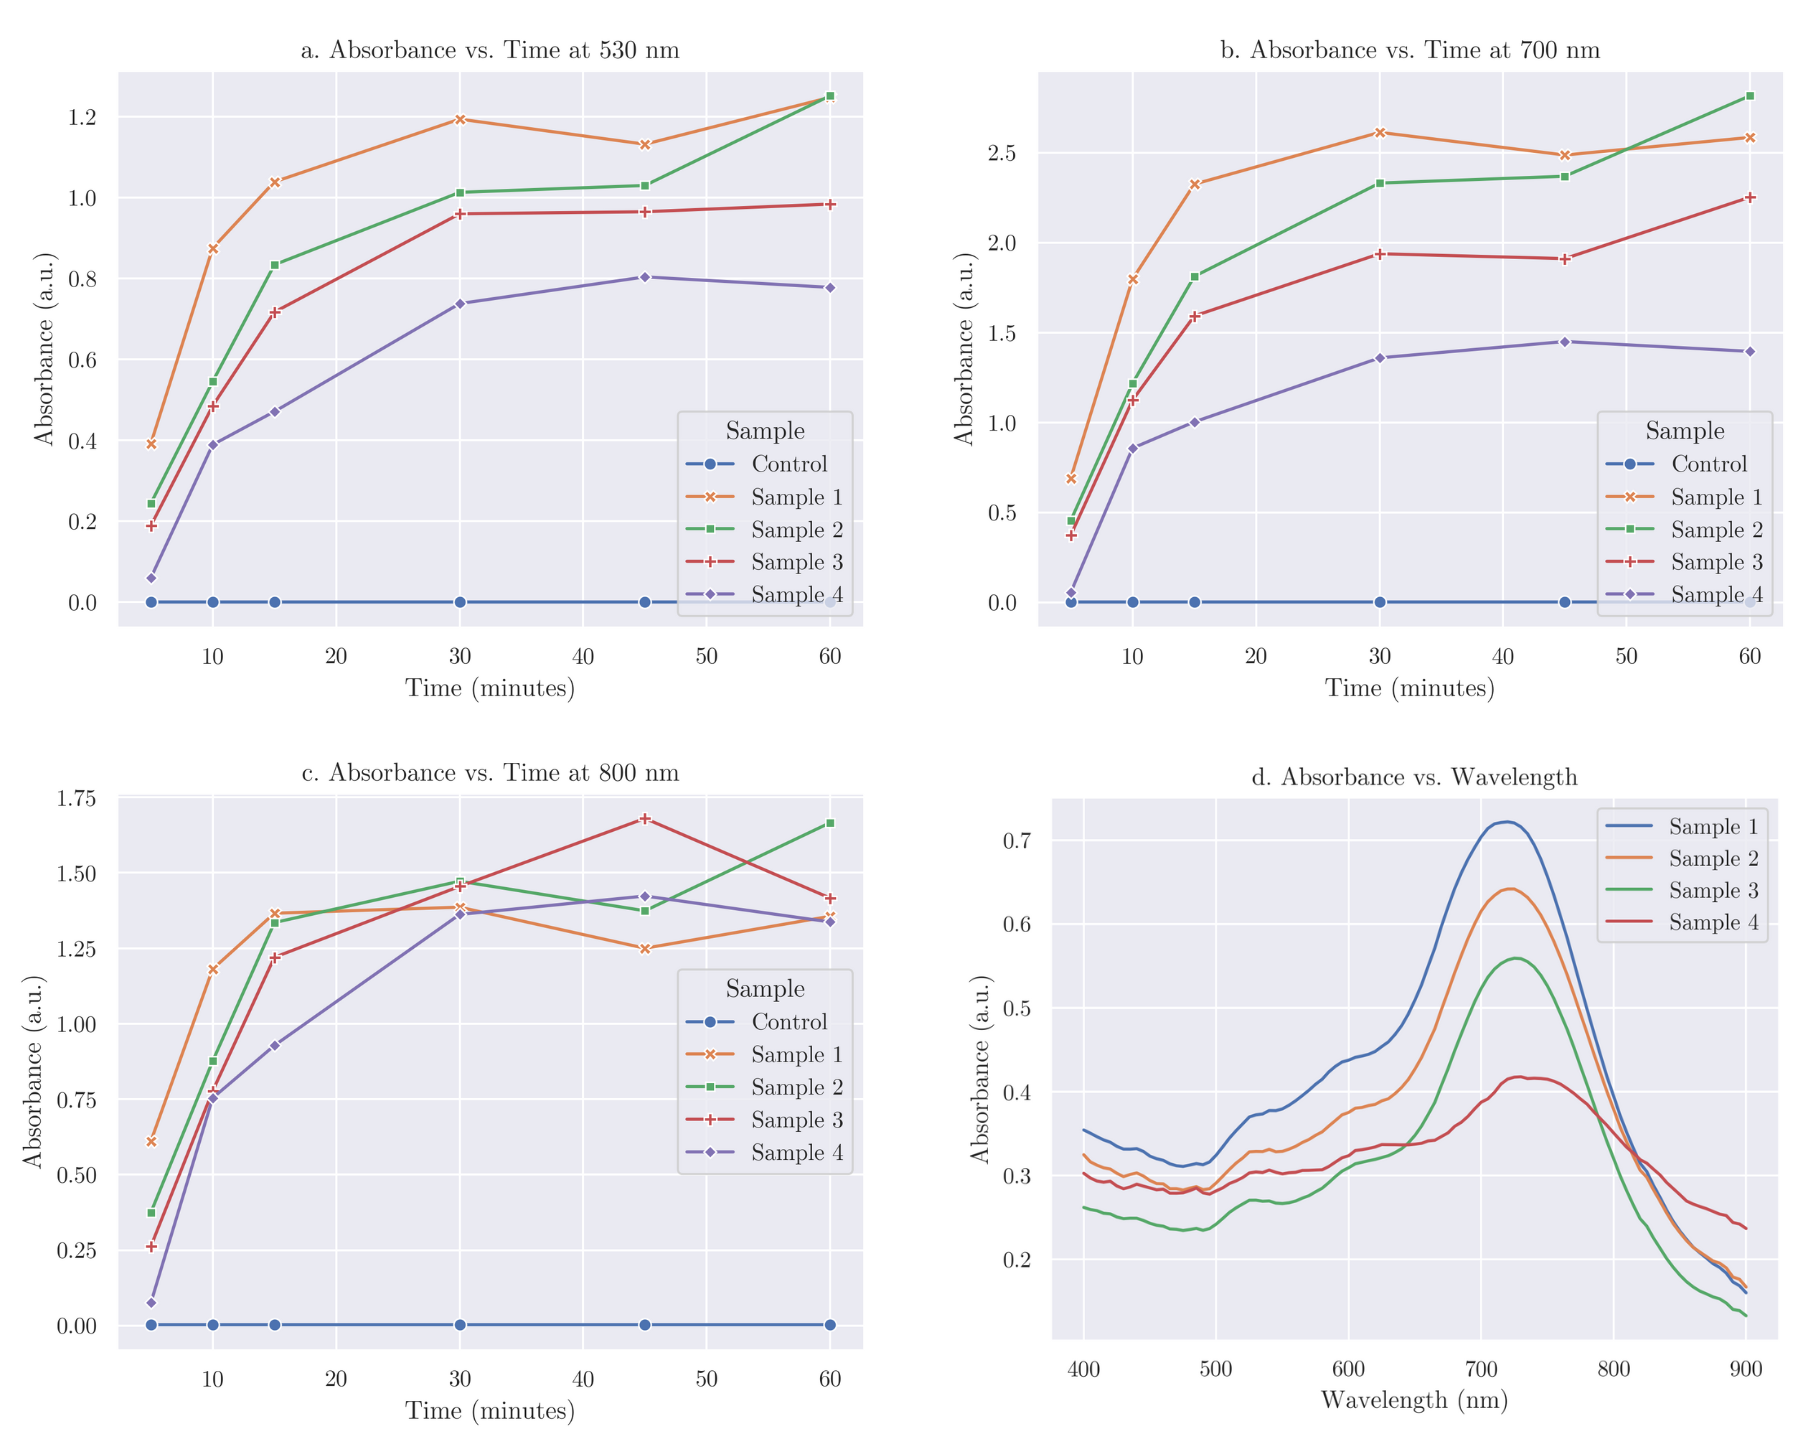
\includegraphics[width=1\textwidth]{data/gn/combined.png}
  \caption{Absorbance values of different samples at different timesteps}\label{fig_gn_1}
\end{figure}

Figure~\ref{fig_gn_1}d clearly shows a collective absorbance peak at $\sim 720$nm which corresponds to an average aspect ratio of $\sim 3.49$ in all samples. This also matches with the data we observe from TEM images. This peak is due to the longitudinal surface plasmon resonance band suggesting a higher concentration of longitudinal mode of gold nanorods. The absorbance values differ significantly for different samples in~\ref{fig_gn_1}d and is higher for the sample with the highest concentration of the seed solution (sample 1) followed by a decrease in absorbance with a decrease in seed concentration. Since the absorbance value is directly proportional to the concentration of nanorods in a solution, this clearly shows that a higher concentration of seed solution allows for a higher concentration/yield of gold nanorods of a similar aspect ratio.

There is a smaller peak at $\sim 520$nm which corresponds to the presence of spherical gold nanoparticles and transversal nanorods. Figures~\ref{fig_gn_1}a-c show that the absorbance values grow with an increase in time and peak at $\sim$ 30 minutes and then stay constant or gradually decrease.

The actual size of the gold nanorods couldn't be calculated theoretically with the collected data as crucial information such as the yield and the concentration of nanorods wasn't known.

This protocol demonstrates that seed-mediated synthesis of Gold nanorods results in a high-quality monodisperse yield of nanorods of an Aspect Ratio of around 3.5 and that seed concentration is directly proportional to the yield of nanorods.

\section{Synthesis of Quantum Dots using Hot Injection}
Ever since the creation of the first \ce{CdSe} Quantum Dots by 2023 Nobel Laureate Dr. Moungi Bawendi\cite{murray1993synthesis} in 1995, these nanoparticles have taken the scientific community by storm. With their unique size-dependent optoelectronic properties, they have found applications in fields like medical imaging, display technology, photovoltaics, etc.

The mechanism of quantum dots can be explained using the `Particle in a Box' model\cite{Modern_Vibrational} which states that the electron confined in an infinite potential well can only attain a discrete set of energy levels. This ensures that the wavefunction equates to zero at the boundaries of the well and is continuous throughout. Assuming `a' to be the width of the well, the energy levels and the wavefunction are given by:
\[\psi_n(x)=\sqrt{\frac{2}{a}} \sin(\frac{n\pi x}{a}); \quad \quad E_n = \frac{\hbar^{2} \pi^{2} n^{2}}{2ma^{2}}; \quad \quad n=1, 2, 3, 4, . . .\]

While light when irradiated upon a quantum dot excites its electrons from the valence shell to the conduction shell leaving a hole behind. This coupling forms a quasiparticle called the \textbf{exciton}. When this exciton recombines, a photon is released with its energy equal to the energy gap between the bands causing smaller quantum dots to emit blue light (higher energy) and larger ones to emit red (lower energy).

In our experiments, two sets of quantum dots were prepared: one using a capping agent, Oleyamine, and one without. In a round bottom flask, 10mL of octacedene was added and put on a heat plate at $165 \degree$ C. In the first batch 1mL each of Cd and Se stock solutions were simulataneously added. At different timestamps, 1mL of the solution was extracted and the growth was halted by putting it in a temporary ice bath. The second batch was prepared identically but with the addition of 0.67mL of Oleyamine just before the injection of CdSe.

\begin{figure}[h!]
  \centering
  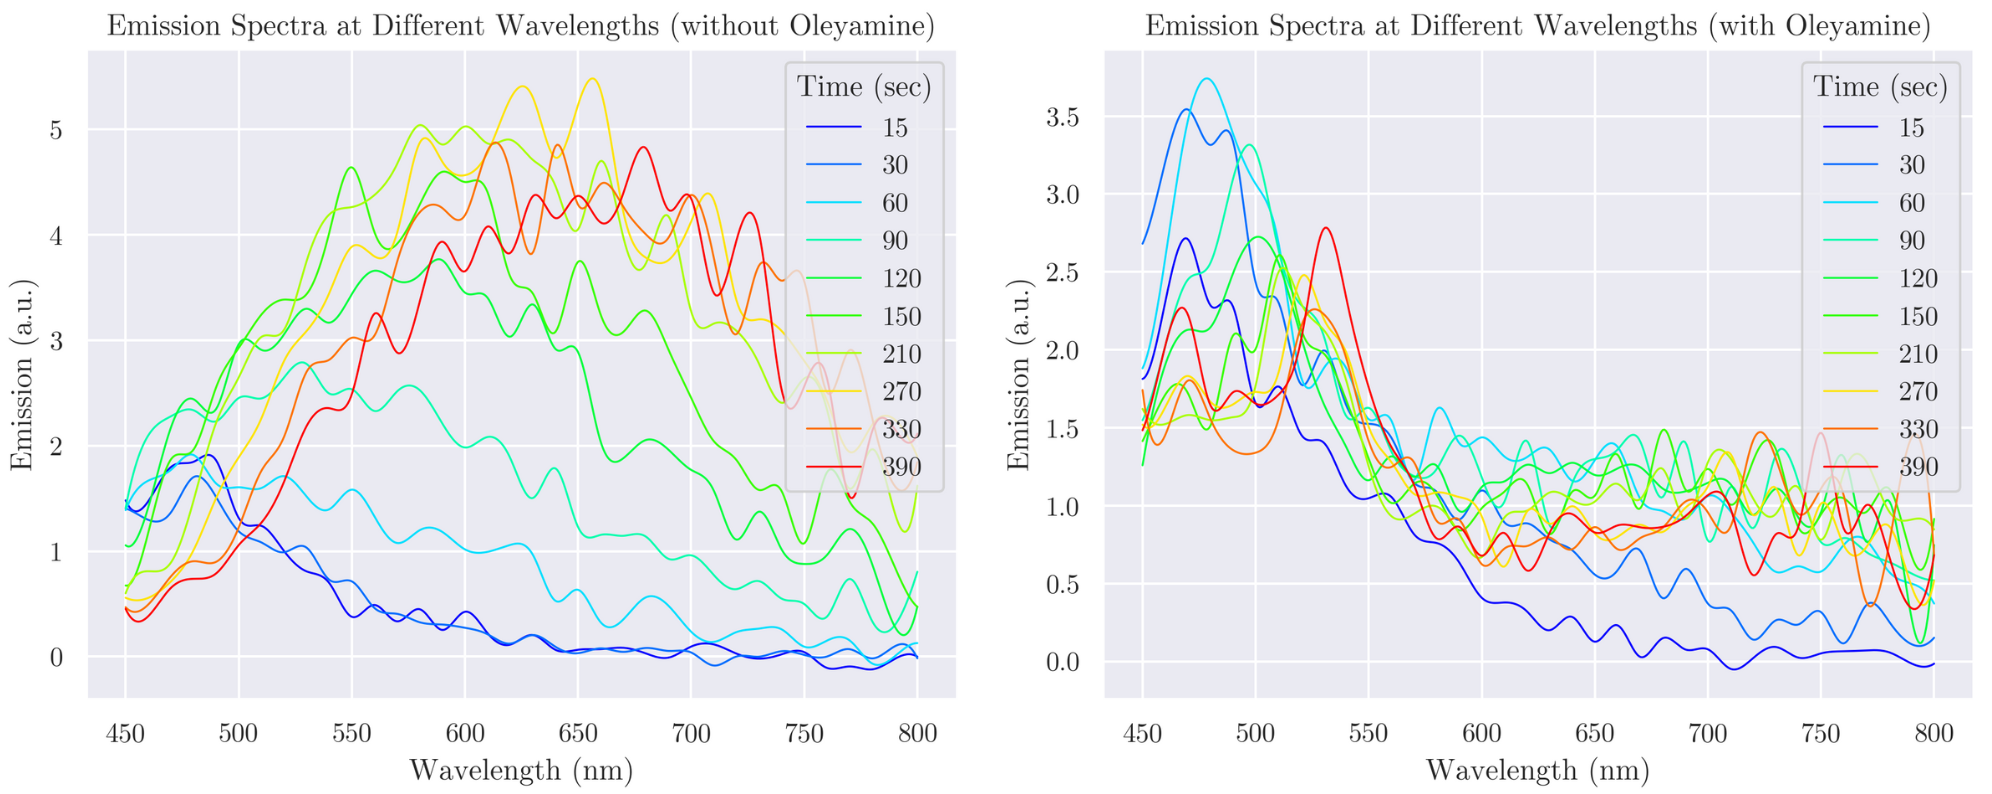
\includegraphics[width=1\textwidth]{data/qds/combined.png}
  \caption{Emission / Fluorescence values of quantum dots at different wavelengths.}\label{fig1}
\end{figure}

\begin{figure}[h!]
  \centering
  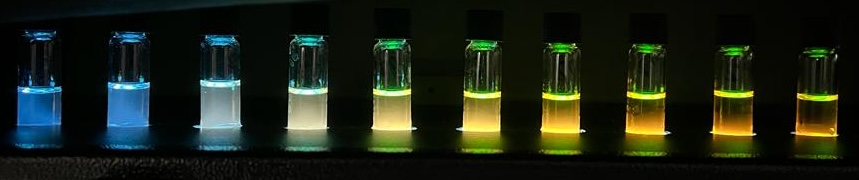
\includegraphics[width=0.9\textwidth]{data/qds/w_o_oleyamine_uv_pic.jpeg}
  \caption{UV Irradiation of Quantum Dots without Oleyamine}\label{fig2}
\end{figure}

Quantum dots display quantum confinement where the electrons probabilistically get confined to a trap state on the surface situated between the conduction and valence band\cite{Landry_Morrell_Karagounis_Hsia_Wang_2013}. The trap state being at lower energy than the conduction band causes the release of a higher wavelength photon causing a wider and more red-shift in the emission peaks as observable clearly from figure~\ref{fig1}a (without Oleyamine). These quantum dots also show bright luminescence under UV light (figure~\ref{fig2}).

As the size of quantum dots increases with time, the emission light shifts from blue to red (\textit{the colors of the curves at different timestamps in figure~\ref{fig1}a and ~\ref{fig1}b represent the actual color observed under UV luminescence.})

Oleyamine acts as a surface capping agent allowing for better stabilization of quantum dots and thus producing an overall smaller and more monodisperse yield\cite{Landry_Morrell_Karagounis_Hsia_Wang_2013}. This directly corresponds to a reduction in redshift as well as trap state confinement. These dots, causally, show mild luminescence under UV light due to low confinement properties. The primary emission source for these particles is exciton recombination. This results in sharper and bluer emission peaks as the energy gap between the conduction and valence band (or an exciton pair) is higher than the energy gap between the trap state and the valence band.

% Cite Brus Equation
The radius of these quantum dots was calculated using the Bruce equation\cite{Modern_Vibrational} and Plank's relation and is summarized for the second batch in the table below.

\[r\left(\lambda \right)=\sqrt{\frac{h^{2}\left(\frac{1}{m_{e}^{*}}+\frac{1}{m_{h}^{*}}\right)}{8\left(\frac{hc}{\lambda }-E_{gap}\right)}}; \quad \quad \Delta E(r) = E_{gap} + \frac{h^{2}}{8r^{2}}\left(\frac{1}{m_{e}^{*}}+\frac{1}{m_{h}^{*}}\right)\]


\begin{table}
  \centering
  \begin{minipage}{0.5\textwidth}
    \centering
    \begin{tabular}{ll}
      \hline
      Time of Withdrawl & Radius  \\
      \hline
      15 seconds        & 2.03 nm \\
      30 seconds        & 2.03 nm \\
      60 seconds        & 2.10 nm \\
      90 seconds        & 2.23 nm \\
      120 seconds       & 2.25 nm \\
      \hline
    \end{tabular}
  \end{minipage}%
  \begin{minipage}{0.5\textwidth}
    \centering
    \begin{tabular}{ll}
      \hline
      Time of Withdrawl & Radius  \\
      \hline
      150 seconds       & 2.32 nm \\
      210 seconds       & 2.34 nm \\
      270 seconds       & 2.41 nm \\
      330 seconds       & 2.47 nm \\
      330 seconds       & 2.54 nm \\
      \hline
    \end{tabular}
  \end{minipage}
  \caption{Radius of Quantum Dots (with Oleyamine) at Different Timestamps}
\end{table}

The calculated radius of the quantum dots linearly increases with the increase in the time of withdrawal as observed by the table above further reinforcing the emission properties of quantum dots elucidated in the figures above.

\bibliography{achemso-demo}

\end{document}